\documentclass[11pt,letterpaper]{article}
\PassOptionsToPackage{hyphens}{url}
\usepackage[margin=.83in,top=.8in,bottom=.8in,headheight=15pt]{geometry}
\usepackage[T1]{fontenc}
\usepackage{lmodern,amsmath,amssymb,mathtools,bm,booktabs,array,graphicx,tikz}
\usetikzlibrary{arrows.meta,positioning,calc,decorations.pathreplacing,patterns}
\definecolor{ink}{HTML}{17344D}\definecolor{accent}{HTML}{087E8B}\definecolor{pale}{HTML}{EDF5F5}\definecolor{gold}{HTML}{AD6B19}
\providecommand{\dd}{\,\mathrm{d}}\providecommand{\R}{\mathbb{R}}
\providecommand{\E}{\mathbb{E}}\providecommand{\Var}{\operatorname{Var}}
\providecommand{\Cov}{\operatorname{Cov}}\providecommand{\diag}{\operatorname{diag}}
\providecommand{\norm}[1]{\left\lVert#1\right\rVert}
\providecommand{\abs}[1]{\left|#1\right|}
\usepackage{microtype,hyperref,fancyhdr,enumitem,amsthm,sectsty,needspace}
\allsectionsfont{\raggedright}
\hypersetup{colorlinks=true,linkcolor=ink,urlcolor=accent,pdfauthor={Zan Ahmad},pdftitle={From image geometry to a tracer balance / Lecture notes}}
\setlength{\parindent}{0pt}\setlength{\parskip}{6pt}\linespread{1.07}
\setlist{itemsep=3pt,topsep=4pt,leftmargin=*}
\emergencystretch=2em\clubpenalty=10000\widowpenalty=10000
\pagestyle{fancy}\fancyhf{}\fancyhead[L]{\small Mathematical Cardiology}\fancyhead[R]{\small Lecture 9}
\fancyfoot[L]{\footnotesize Zan Ahmad}\fancyfoot[R]{\footnotesize\thepage}\renewcommand{\headrulewidth}{.3pt}
\newtheorem{proposition}{Proposition}\newtheorem{theorem}{Theorem}\newtheorem{lemma}{Lemma}
\theoremstyle{definition}\newtheorem{definition}{Definition}\newtheorem{example}{Example}
\numberwithin{equation}{section}
\begin{document}
{\small\scshape Mathematical Cardiology\hfill Lecture 9}\par\medskip
{\raggedright\hyphenpenalty=10000\exhyphenpenalty=10000\LARGE\bfseries\color{ink} From image geometry to a tracer balance\par}\medskip
{\small Lecture notes}\par\bigskip
A region that appears poorly connected in an image suggests a question about exchange, but the image does not contain a flow field. We shall distinguish the geometric operations that define a region from the conservation law that predicts a tracer concentration. The resulting washout model is small enough to solve exactly. Its most useful limitation is equally exact: one concentration cannot describe a difference between a main chamber and a side pocket.

\section{An intensity field and a selected region}
\hypertarget{note-an-intensity-field-and-a-selected-region}{}\label{note:an-intensity-field-and-a-selected-region}
{\small \href{slides.html\#frame=a-picture-contains-intensities-figure\&step=1}{Slides for this section}}\par
Represent a grayscale image by numbers $I_{ij}$ arranged on a pixel grid. The companion creates a synthetic chamber, side pocket and two openings, blurs their boundary, and adds a small random intensity perturbation. None of these pixels is a patient measurement. A threshold $\theta$ defines the mask
\begin{equation}M_{ij}(\theta)=\begin{cases}1,&I_{ij}\geq\theta,\\0,&I_{ij}<\theta.\end{cases}\end{equation}
Its selected pixel count is $N(\theta)=\sum_{ij}M_{ij}(\theta)$. If $\theta_2>\theta_1$, every pixel selected at $\theta_2$ is also selected at $\theta_1$. Therefore $N(\theta_2)\leq N(\theta_1)$. This is a consequence of the threshold definition, not an empirical discovery about anatomy.

In the displayed image, thresholds $0.4$, $0.5$ and $0.6$ select $1699$, $1641$ and $1563$ pixels. The ordering checks the implementation. It cannot tell us which boundary is physically correct. If the pixel spacings are $s_x,s_y$, an area estimate is $A=N s_xs_y$. A volume estimate needs out-of-plane information; even an exact two-dimensional contour is insufficient. The default image's normalized drawing coordinates are not a measured millimeter scale.
\begin{center}\begin{minipage}{.98\linewidth}\centering
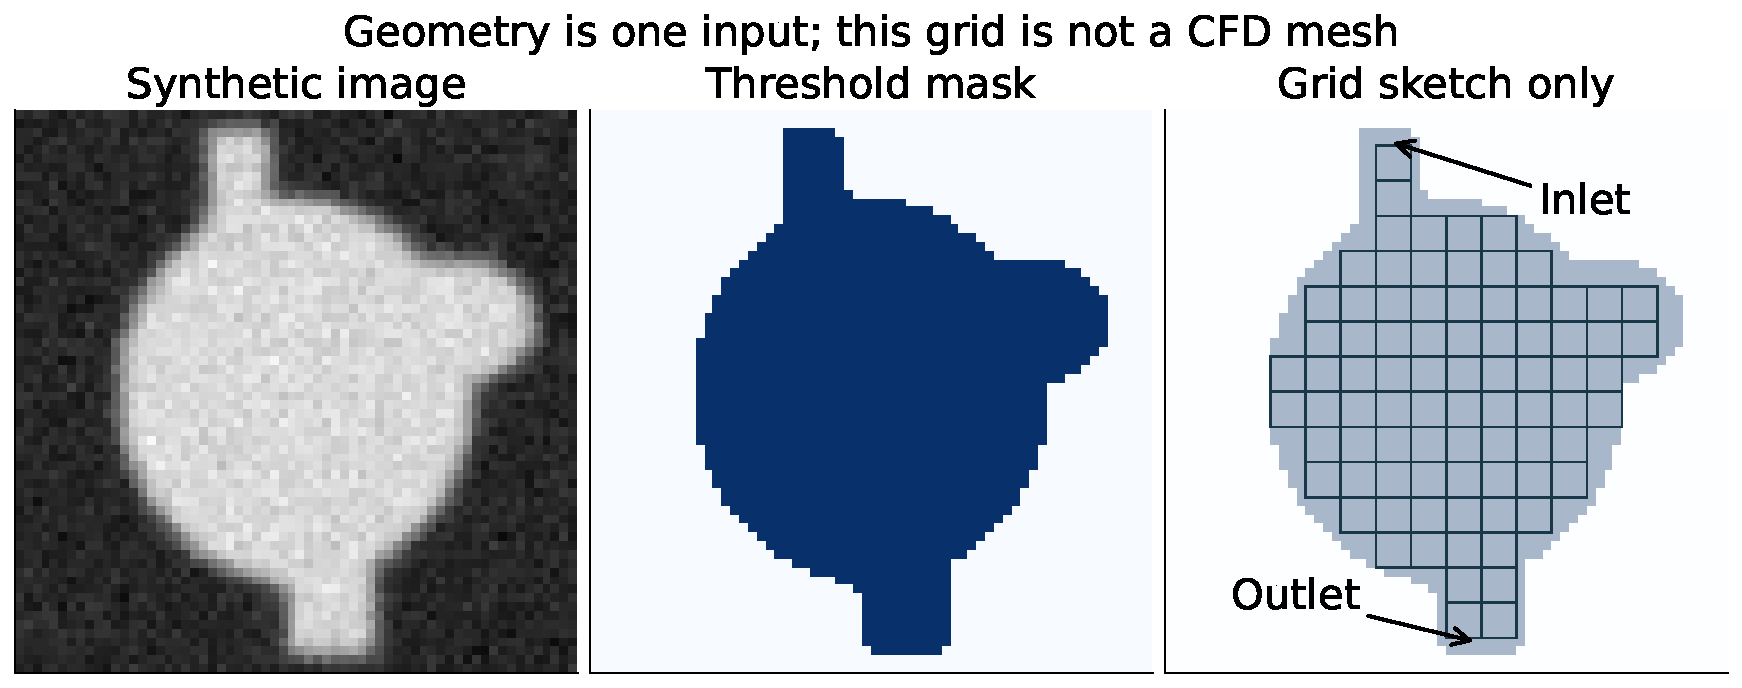
\includegraphics[width=.96\linewidth,height=.57\textheight,keepaspectratio]{image-pipeline.pdf}\par\smallskip
{\small Original synthetic intensity image, threshold mask and interior square-grid sketch. The top and bottom labels mark invented openings. This is not patient anatomy or a CFD mesh.}
\end{minipage}\end{center}
\section{Connectivity and the missing spatial problem}
\hypertarget{note-connectivity-and-the-missing-spatial-problem}{}\label{note:connectivity-and-the-missing-spatial-problem}
{\small \href{slides.html\#frame=a-small-area-change-can-alter-a-route\&step=1}{Slides for this section}}\par
Area is not the only geometric quantity that matters. Removing a small set of pixels at the side-pocket neck can disconnect the pocket while barely changing the area. The top and bottom openings must likewise survive segmentation and receive explicit boundary labels. Smoothing a contour can enlarge or remove a narrow route; a visually smoother surface is not automatically a more faithful one.

The third figure panel retains square cells lying entirely inside the mask. It demonstrates spatial subdivision, but it omits cut boundary cells and does not certify a solver-ready mesh. For this particular drawing, a spatial model would first need physical spacing, a connected pocket neck, an identified top inlet, an identified lower outlet, and wall labels on the remaining boundary. A suitable volume mesh would then need enough resolution near narrow features and consistent connectivity.

Conservation applies locally in a spatial flow model. For a fixed, incompressible cell, signed volume fluxes through its faces sum to zero:
\begin{equation}\sum_{f\in\partial\text{cell}}Q_f=0,\end{equation}
where outward flux is positive. Shared-face fluxes cancel when neighboring cells are added, leaving only the external boundary flows. This is the same cancellation used in our circulation networks, now repeated over many small volumes. It supplies a constraint, not a complete velocity solution: momentum balance, fluid properties, boundary conditions and perhaps wall motion must also be specified. The SimVascular paper describes an image-to-flow pipeline with these additional modeling stages; it is background for the workflow, not evidence that this grid sketch solves flow.
\section{A deliberately well-mixed reduction}
\hypertarget{note-a-deliberately-well-mixed-reduction}{}\label{note:a-deliberately-well-mixed-reduction}
{\small \href{slides.html\#frame=reduce-the-region-to-one-mixed-volume\&step=1}{Slides for this section}}\par
We now discard the spatial subdivision and retain one constant volume $V$. Let $C(t)$ be tracer amount per unit fluid volume, so the total tracer amount is $M(t)=VC(t)$. The inlet carries flow $Q$ with tracer concentration $C_{\rm in}$, and the outlet carries the same flow with concentration $C(t)$. Equality of inlet and outlet flow keeps the fluid volume constant. Complete mixing makes the outlet concentration equal to the single compartment concentration.

Over a short interval $h$, holding the current concentration fixed for the calculation gives
\begin{equation}M(t+h)-M(t)\simeq hQ C_{\rm in}-hQ C(t).
\end{equation}
For tracer-free inflow, $C_{\rm in}=0$. Dividing by $V$ gives the explicit update
\begin{equation}C_{n+1}=\left(1-\frac{hQ}{V}\right)C_n.\label{eq:washout-step}\end{equation}
The multiplier is dimensionless. This finite-step approximation preserves a nonnegative concentration when $0\leq hQ/V\leq1$. A negative numerical concentration from a larger step would reflect the update, not a physical creation of negative tracer. The supplied companion evaluates the exact curve instead; this recurrence is a derivation and a numerical comparison, not the implemented solver.
\section{The exponential and its time scale}
\hypertarget{note-the-exponential-and-its-time-scale}{}\label{note:the-exponential-and-its-time-scale}
{\small \href{slides.html\#frame=repeated-removal-gives-an-exponential\&step=1}{Slides for this section}}\par
As the interval becomes small, the balance becomes
\begin{equation}V\frac{\mathrm dC}{\mathrm dt}=-QC,\qquad C(0)=C_0.
\end{equation}
The derivative means the instantaneous rate of concentration change. For $Q>0$, the solution and its time constant are
\begin{equation}\frac{C(t)}{C_0}=e^{-Qt/V}=e^{-t/\tau},\qquad \tau=V/Q.\label{eq:washout-exact}\end{equation}
One can understand the exponential without solving a differential equation: with $n$ equal intervals in a fixed time $t$, equation \eqref{eq:washout-step} gives the fraction $(1-Qt/(nV))^n$. As the intervals become finer this tends to $e^{-Qt/V}$. The shrinking removal in successive intervals reflects dilution; a constant amount of tracer is not removed each second.

For $V=100\,\mathrm{mL}$ and $Q=25,50,100\,\mathrm{mL/s}$, the time constants are $4,2,1\,\mathrm{s}$. At $t=2\,\mathrm{s}$ the remaining fractions are respectively $e^{-1/2}\simeq0.607$, $e^{-1}\simeq0.368$ and $e^{-2}\simeq0.135$. The half-time solves $e^{-t_{1/2}/\tau}=1/2$, giving $t_{1/2}=\tau\log2$. In particular, the time constant is not the half-time.

If $Q=0$, the original balance gives $C(t)=C_0$; there is no washout. One should use that limiting equation rather than divide by zero in $\tau=V/Q$. Multiplying both $V$ and $Q$ by the same positive factor leaves every fraction unchanged. Thus a concentration-decay curve determines the ratio $Q/V$, not both quantities separately.
\begin{center}\begin{minipage}{.98\linewidth}\centering
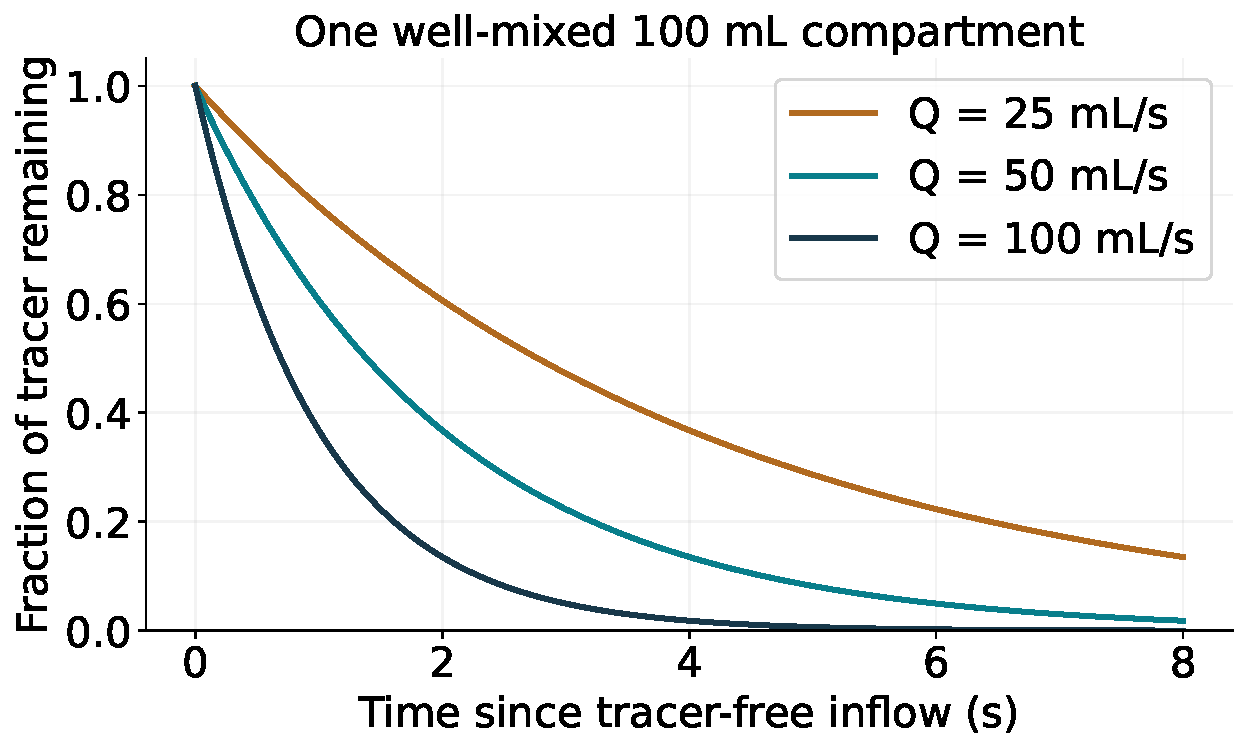
\includegraphics[width=.96\linewidth,height=.57\textheight,keepaspectratio]{washout.pdf}\par\smallskip
{\small Exact exponential washout in one well-mixed 100 mL compartment at three prescribed balanced flows. The curves contain no spatial velocity, wall shear or clot prediction.}
\end{minipage}\end{center}
\section{A separate concentration state for the pocket}
\hypertarget{note-a-separate-concentration-state-for-the-pocket}{}\label{note:a-separate-concentration-state-for-the-pocket}
{\small \href{slides.html\#frame=a-pocket-needs-its-own-state\&step=1}{Slides for this section}}\par
The well-mixed model assigns the same $C(t)$ to the pocket and main chamber by definition. It therefore cannot discover a slowly exchanging pocket. An optional extension shows exactly what is missing. Let $V_a,C_a$ describe a main chamber and $V_b,C_b$ a pocket. Let an external tracer-free flow $Q$ pass through the main chamber, and let $q$ be equal bidirectional exchange between the two compartments. Then
\begin{align}
V_a\frac{\mathrm dC_a}{\mathrm dt}&=-QC_a+q(C_b-C_a),\\
V_b\frac{\mathrm dC_b}{\mathrm dt}&=q(C_a-C_b).
\end{align}
Adding the balances cancels the internal exchange:
\begin{equation}\frac{\mathrm d}{\mathrm dt}(V_aC_a+V_bC_b)=-QC_a.\end{equation}
This is an illustrative extension in the notes; it is not computed by the companion. When $q=0$, tracer in the pocket remains there even as the main chamber washes out. If the pocket initially contains tracer, the total tracer need not decay to zero. The one-compartment assumption has removed the very state variable needed to represent this possibility. The drawing alone supplies neither $q$ nor a justification for complete mixing.
\section{Numerical refinement and independent validation}
\hypertarget{note-numerical-refinement-and-independent-validation}{}\label{note:numerical-refinement-and-independent-validation}
{\small \href{slides.html\#frame=two-different-tests\&step=1}{Slides for this section}}\par
A spatial simulation of the synthetic chamber would require a specified inflow profile or waveform at the top opening, an outlet pressure or pressure--flow relation at the lower opening, wall-motion or rigid-wall assumptions, and fluid properties. These choices influence the result even if the mask is held fixed. A mesh-refinement check should retain the same physical assumptions and compare a named output, such as an outlet tracer curve, across successively finer meshes and time steps. Agreement tests sensitivity to numerical resolution. Independent measurements of that output test whether the physical model is adequate.

The exact washout calculation supports a precise statement: for fixed positive $V$ and positive time, decreasing prescribed $Q$ leaves more tracer in a perfectly mixed compartment. It supplies no spatial velocity, wall shear or location-specific residence pattern. A connection to clot formation or stroke requires biological and outcome evidence beyond a concentration curve. For a pocket-specific exchange claim, the first missing ingredient is already mathematical: a model that can distinguish pocket concentration from main-chamber concentration, together with evidence for its exchange parameters.
\bigskip
\section*{Exercises}
\par\noindent\begin{minipage}{\linewidth}
\subsection*{MC09-E1. Threshold and physical area}
A synthetic image has square pixels 2 mm on a side. One threshold selects 300 pixels; another selects 330.

\textbf{a} Calculate both selected areas.

\end{minipage}\par\medskip
\textbf{b} Compute the relative area change from the first selection.

\textbf{c} Explain why this does not determine chamber volume.

\par\noindent\begin{minipage}{\linewidth}
\subsection*{MC09-E2. A different washout scale}
A well-mixed 160 mL compartment has balanced tracer-free inflow/outflow of 40 mL/s.

\textbf{a} Find the time constant and remaining fraction at 4 seconds.

\end{minipage}\par\medskip
\textbf{b} What happens if both volume and flow double?

\textbf{c} What information is lost by assuming perfect mixing?

\par\noindent\begin{minipage}{\linewidth}
\subsection*{MC09-E3. Inspect the displayed workflow}
Use the synthetic image-pipeline figure.

\textbf{a} Name three geometric checks before attempting spatial simulation.

\end{minipage}\par\medskip
\textbf{b} Name three missing physical inputs.

\textbf{c} Design a numerical refinement comparison and distinguish it from validation.

\par\noindent\begin{minipage}{\linewidth}
\subsection*{MC09-E4. Repair an overclaim}
A report states: ``The curve decays more slowly, so this patient will have a stroke.''

\textbf{a} List two unsupported links in this statement.

\end{minipage}\par\medskip
\textbf{b} Rewrite a claim supported by the demonstration.

\textbf{c} Name additional evidence needed for a stronger spatial claim.

\section*{References}
\noindent\begin{minipage}{\linewidth}
Zan Ahmad, Mathematical Cardiology syllabus, Fall 2023. Public PDF pages 1--2, Course Topics and Course Objectives.

\url{https://zanahmad.com/files/Fall_2023_HEART_Syllabus.pdf}
\end{minipage}\par\medskip
\noindent\begin{minipage}{\linewidth}
Zan Ahmad, original editable Mathematical Cardiology syllabus. Rendered export pages 2--3, Assignments \& Grading and Projects.

\end{minipage}\par\medskip
\noindent\begin{minipage}{\linewidth}
Updegrove, Wilson, Merkow, Lan, Marsden and Shadden, SimVascular: An Open Source Pipeline for Cardiovascular Simulation (2017). Methods: The SimVascular Pipeline; Meshing; Simulation---Boundary Conditions, Inlets, Outlets; DOI 10.1007/s10439-016-1762-8; sections read 2026-11-14.

\url{https://pmc.ncbi.nlm.nih.gov/articles/PMC6546171/}
\end{minipage}\par\medskip
\noindent\begin{minipage}{\linewidth}
NHLBI, What Is Atrial Fibrillation?. Overview and discussion of blood pooling, clots and stroke; page dated 2022-11-30, read 2026-11-14.

\url{https://www.nhlbi.nih.gov/health/atrial-fibrillation}
\end{minipage}\par\medskip
\end{document}
